\documentclass[12pt]{report}
\usepackage[utf8]{inputenc}
\usepackage{graphicx}
\usepackage{tabularx}
\usepackage{listings}
\usepackage{hyperref}
\usepackage{microtype}
\usepackage{flushend}
\usepackage{amsmath}
\usepackage{booktabs}
\usepackage{bibentry}
\usepackage[backend=biber,style=alphabetic,sorting=ynt]{biblatex}

%\usepackage{physics}
\usepackage{mathdots}
\usepackage{yhmath}
\usepackage{cancel}
\usepackage{color}
\usepackage{siunitx}
\usepackage{array}
\usepackage{multirow}
\usepackage{amssymb}
\usepackage{gensymb}
\usepackage{extarrows}
\usepackage{tikz}
\usetikzlibrary{fadings}
\usetikzlibrary{patterns}
\usetikzlibrary{shadows.blur}
\usetikzlibrary{shapes}
\tikzset{every picture/.style={line width=0.75pt}} %set default line width to 0.75pt 

\addbibresource{thesis.bib}

% Tech Dims
\usepackage{changepage} % For the single-page summary table PDF insert.
\usepackage{pdfpages}
\usepackage{pifont} % For checkmark / cross symbols for Appendix table :)
\usepackage{amsthm} % For numberless Definition
\usepackage{epigraph} % For the opening quotes

\graphicspath{{../img/}}

\lstset{breaklines=true, columns=fullflexible, breakatwhitespace=true, basicstyle=\ttfamily\footnotesize}
\lstdefinelanguage{JavaScript}{
  keywords={break, case, catch, continue, debugger, default, delete, do, else,
  finally, for, function, if, in, instanceof, new, return, switch, this, throw,
  try, typeof, var, void, while, with, let, false, true},
  morecomment=[l]{//},
  morecomment=[s]{/*}{*/},
  morestring=[b]',
  morestring=[b]",
  sensitive=true
}
\lstset{
  language=JavaScript,
  numbers=none,
  columns=fullflexible,
  basicstyle=\ttfamily,
}

\title{
  {Achieving Self-Sustainability in Interactive Graphical Programming Systems}\\
  {\large University of Kent}
}
\author{Joel Jakubovic}

\begin{document}
\maketitle

\newcommand{\joel}[1]{}
\newcommand{\tomas}[1]{}
\newcommand{\tp}[1]{}
\newcommand{\note}[1]{}
\newcommand{\notes}[1]{}
\newcommand{\todo}[1]{\textbf{TODO: #1}}
\newcommand{\delete}[1]{\textbf{DELETE:}#1}
\newcommand{\naive}{na\"ive}
\newcommand{\OROM}{Id}
\newcommand{\svgel}[1]{\texttt{\textless{}#1\textgreater{}}}
\newcommand{\RTFJ}{Right Tool For The Job}
\newcommand{\URTFJ}{Use The \RTFJ}
\newcommand{\OSFA}{One-Size-Fits-All}
\newcommand{\xywh}{\texttt{x},\texttt{y},\texttt{width},\texttt{height}}
\newcommand{\criterion}{\paragraph}
% Thanks https://tex.stackexchange.com/a/32687
\NewDocumentCommand{\rot}{O{45} O{1em} m}{\makebox[#2][l]{\rotatebox{#1}{#3}}}%
\newcommand{\mybox}[1]{\noindent\fbox{\parbox{\textwidth}{#1}}}
\providecommand{\tightlist}{}% Don't want Pandoc's tight lists
% Nor do we want long tables by default
\newenvironment{longtable}[2]{\begin{tabular}}{\end{tabular}}
\newenvironment{head}{}{}
%\newcommand{\hypertarget}[1]{}
\newtheorem{heuristic}{Heuristic}
\newtheorem{defn}{Definition}

\input{ch-preamble.tex}
\chapter{Introduction}

\note{in html/dom - you can open object browser and edit user interface, but this does not work for editing code in the same way - that is bulk JS with some substrings you would have to edit; what if everything was visible accessible (shareable) and editable, including structured code?

if I want to draw GUI, I can either write code or use GUI editor like VB or Hypercard - but the GUIs exist as separate to the programming system - could they be integrated like DSLs?

third - maybe COLA or Smalltalk - do self-sustainability but not quite.

Capabilities:
* Create (author) static content. static authoring. Hc, St
* Create (author) dynamic content. dynamic authoring. Hc, St
* Make a small change without having to restart the world. (self-sus) pokeability
* Change structural state without having to re-build the structure. (parsing bad) static pokeability. Hc St Web
* Change behavioural state without having to re-build the behaviour. dynamic pokeability Hc St
* Domain-specific notations. COLA

1. what is your quest - for a non-computer person
2. many pieces of the puzzle exist - web, hypercard, smalltalk
3. why hasn't anyone done this? PL paradigm is wrong - we need systems
4. systems allow better thinking! here is more specifically what I'm working on
}

\joel{
These concerns point to an unexplored opportunity which constitutes the contribution of this thesis. We discuss how the Three Properties feed into each other and hence why we study them together. We close with a summary of what the thesis contribution is.
}

When we have an idea for some computer software, and try and make this
idea a reality, we are forced to confront two types of complexity: the
\emph{essential} and the \emph{accidental}. We know there is ``no such
thing as a free lunch'', so we are able to accept the burden of whatever
complexity is actually intrinsic to our idea. If we have a simple idea,
we are prepared to do a little work; if it is more ambitious, we will
accept having to do more work. This \emph{essential} complexity is often
swamped by unwelcome incursions of tedious busy-work. Concepts that
appear simple must be spelled out in great detail for a computer. This
is the \emph{accidental complexity} that is widespread in programming
\cite{MMM}.

This is particularly egregious when the ``idea'' is merely to change or
fix some small issue. Suppose we are using an app, but the text is too
small for us to read. The designers have not included a feature for
increasing the text size (perhaps it is a special message in a separate
part of the app which is unaffected by the normal controls). A
programmer would know that there is some API being called to render the
text, and this API will be told the font size via some number in the
app's memory. If we could just find this single number and change it, we
might at least be able to read the text (even if the app is not prepared
to lay out the larger text correctly in response to such a ``surgical''
intervention).

So, what does it take to find and change a number? The app itself
provides no way to proceed through its surface interface to such
internal details. This means we must face at least the accidental
complexity of working with some external tool that can open it up. We
could attach an assembly-level debugger to the app process and stare at
hex dumps for a long time, eventually figuring out which address holds
the font size. Such an expert task would take an extremely long time
even for someone with the relevant experience. It does let us make a
change to the running app, but not permanently; we would have to do this
every time we ran the app.

Alternatively, we could hope that the app is open-source, download the
code, setup the build system, locate the relevant code, re-build the
app, and re-install it. Each of these steps is also an expert task which
would be incredibly lengthy, even for programmers, on a novel codebase.
Furthermore, this approach entails destroying the running instance of
the app and re-initialising it, possibly losing unsaved work.

In the worst case, both of these approaches could be blocked; run-time
tampering could be prevented by security policy (especially on a mobile
device) and re-building from source cannot work without access \emph{to}
the source. Suffice to say, none of this is suitable for an average
user. Even a seasoned programmer would consider it not worth the bother.
Our task of changing a number, while technically possible, has a
severely \emph{disproportionate} accidental complexity cost.

In specific situations, software authors do have good reasons to
restrict access to internals. For example, in a game it is important to
enforce the rules and access to internals would enable arbitrary
cheating. However, this consideration is not representative of most
types of software. Despite this, we are unable to simply \emph{choose}
to build such ``open'' software. Even if \emph{we} wrote the app and
desire to support adaptation beyond what we anticipated, we face the
fact that our tools can only create software that is ``closed''. The
task of ``supporting unanticipated modification'' is itself a
\emph{feature} that we must somehow figure out and implement on top, and
it is unclear how to achieve such a feature. Nevertheless, it is worth
striving for a world where this accidental complexity is as reduced as
possible. We might expect this to involve a mix of ``demolition''
work---that of removing barriers that have been placed in the way---and
``construction'' work of building tools that help us work more
effectively.

\hypertarget{how-should-things-work}{%
\section{How Should Things Work?}\label{how-should-things-work}}

Imagine a world where the average computer user can patch or improve
their software the same way they might change a lightbulb or perform DIY
in their home. This clearly relies on the ability to make small
\emph{piecemeal} changes to their home, without having to demolish the
place and re-build it anew. Let's call this \emph{naïve pokeability}:

\begin{defn}[Naïve pokeability]
\label{def:naive-pokeability}
A change has \emph{naïve pokeability} if it is possible to make the change while the software is \emph{running} without having to consider the implications of restarting it.
\end{defn}

Furthermore, the common-sense expectation is that the changes
\emph{persist} into the future:

\begin{defn}[Persistent]
\label{def:persistent}
The result of a change is \emph{persistent} if it remains until a future change overrides its effect.
\end{defn}

\begin{defn}[Transient]
\label{def:transient}
A change is \emph{transient} if, in the absence of special measures, it will be undone within a short timeframe and its effects will not last.
\end{defn}

Additionally, the tools for making changes are of an appropriate scale
and reside within the system. Changes are \emph{self-supplied} and, if
this covers all possible changes, we have a \emph{self-sustainable}
environment.

\begin{defn}[Self-supplied]
\label{def:self-supplied}
A change is \emph{self-supplied} by a piece of software if you can achieve the change by only using the software.
\end{defn}

\begin{defn}[Self-sustainable]
\label{def:self-sustainable}
A software system is \emph{self-sustainable} if arbitrary changes to it are self-supplied.
\end{defn}

The system functions like a workshop where new tools can be fashioned
using existing tools as needed. They can be big or small, and this
ensures that we can use the ``right tool for the job'', no matter the
scale.

\begin{defn}[\RTFJ]
\label{def:right-tool}
This is a principle in programming which acknowledges that tools have differing strengths and weaknesses for different tasks. To ``\URTFJ'' is an ideal that relies on either an existing range from which to select the best tool or the capacity to design and build it on-demand.
\end{defn}

\begin{defn}[One-Size-Fits-All]
\label{def:osfa}
The opposite of ``\URTFJ''. This refers to using a single tool to do a wide range of tasks even though it may not be suited for some of them.
\end{defn}

\begin{defn}[Domain-Specific Adaptation]
\label{def:dsa}
This is a small or large part of a software system which provides its own custom interface for change.
\end{defn}

In standard practice, a program is generated from \emph{source code} and
put into a running state. To change the program, one must change the
source code, destroy the program and re-create it anew. These steps are
accomplished with separate tools, meaning that changes tend not to be
self-supplied (Definition~\ref{def:self-supplied}). There is a limited
notion of ``\URTFJ'' in that there are different programming languages.
However, languages enforce their syntax and semantics without permitting
\emph{smaller-scale} adaptation, and variation in these respects is
restricted to textual notations. Furthermore, some situations may call
for more general \emph{notations} or graphical interfaces that do not
work like a language, but fact that programming is optimised for
languages makes using such notations more difficult.

Instead of the above, computer software should act as ``Personal Dynamic
Media'' \cite{PersonalDynMedia}. In this vision, a software system is
\emph{designed} to be adapted and modified by its users. By performing
an explicit action (e.g.~switching to ``edit mode'') the user can
inspect the visible surface of the application to find the causes of its
appearance in the form of code and data. They can also inspect a map of
the non-visible implementation of the software's functionality and
navigate to the relevant parts. There may be a common programming
notation as a default, but where possible, parts of the implementation
are presented in local notations or interfaces that are more easily
understood. These interfaces can also be traced to \emph{their}
implementations and modified if desired. The user can then change any
aspect of the software while it is running, without having to edit an
external specification and destroy the running instance.

\hypertarget{a-fragmented-vision}{%
\section{A Fragmented Vision}\label{a-fragmented-vision}}

Several pieces of this vision do exist, but not in an integrated whole.
We can see some of the different characteristics we desire in software
by discussing the examples of the Web, HyperCard, and Smalltalk.

\hypertarget{web-pages-web-apps-and-browsers}{%
\subsection{Web pages, web apps, and
browsers}\label{web-pages-web-apps-and-browsers}}

The \emph{web browser} has a powerful set of \emph{developer tools}.
This includes the ``element inspector'' which can be used to edit the
web page's underlying elements. For example, an ad can be removed by
locating and deleting its element. Note that the ``state'' here is
mostly visible, since it is directly responsible for visual elements
appearing on the page. Some of the state may have no visual effects
(e.g.~an element's ID attribute) and is thus hidden from an ordinary
user. However, such state is visible from the inspector in the developer
tools. This means that all of the ``structural'' state is
\emph{potentially} visible, not to mention editable, in the web browser.

The above is worth contrasting with the case of the ``behavioural'' side
of a web page centered around the JavaScript programming language.
Alongside the ``structural'' state of the web page, there is also the
hidden state of JavaScript objects. The JavaScript console accepts
commands which may read or change this state, but there is nothing like
the element inspector for it.\footnote{This may be because the ``DOM''
  is a tree structure while the JavaScript state is a general graph, and
  it's harder to build an editor for the latter.} What \emph{is} visible
in the dev tools is the \emph{source code} of the scripts loaded by the
page.

Many changes to the ``behavioural'' state can be accomplished at the
console; for example, updating part of the state to a new object.
However, this will not work if the source declares the variable as
\texttt{const}, and more importantly, this does not work for
fine-grained changes to code. The main unit of code organisation, the
\texttt{function}, is an opaque object in the runtime environment; one
cannot simply replace a particular line or expression within it.
Instead, a complete new definition must be entered into the console to
replace it wholesale. However, replacing a function can be prohibited by
the source just like the redefinition of \texttt{const} variables. In
these cases, there is no choice but to edit the source files somehow. If
the browser does not provide for local edits to be made to these files,
a separate text editor must be used. The changes made in this way do not
take effect until the scripts are reloaded by refreshing the page.

Compare the above situation with the ``structural'' state of the web
page; we are free to make arbitrarily fine-grained changes using the
element inspector, and our changes take effect immediately without
having to reset anything. There are, in fact, HTML text files backing
the page structure, but they are irrelevant given the inspector tool. In
short, the \emph{state} of a web page has \emph{naïve pokeability}
(Definition~\ref{def:naive-pokeability}) while its dynamic
\emph{behaviour} does not reliably have this property.

There is one caveat: since the HTML and JavaScript files are the
``ground truth'', any changes made via the inspector or the console will
disappear when the page is closed or refreshed. Only changes to the
underlying files are \emph{persistent}, and websites typically do not
allow random individuals to change the files on their servers. All this
is sad news for our user deleting their ad, as they will have to repeat
it each time they access the page (or use sophisticated programmatic
middleware, such as an ad-blocking extension, to do this automatically).

\hypertarget{hypercard}{%
\subsection{HyperCard}\label{hypercard}}

Before the Web, ``hypertext'' was regularly created and distributed by
people in the form of HyperCard stacks. Alan Kay criticised the web for
having a browser that doesn't include an \emph{authoring} tool,
instantly limiting the \emph{creation} of web pages to people who can
code in a text editor. In HyperCard, the viewer and editor exist
integrated together. Furthermore, there is an ``edit'' mode whereby a
user can remix content from someone else, even reprogramming the dynamic
behaviour.

These aspects of HyperCard's design encouraged a community of
producer-consumers for hypertext content. The web's higher cost of
authoring led to a lower producer-to-consumer ratio, restricting the
kind of medium that it would become. Note that the naïve pokeability of
the element inspector does not amount to authoring a web page; such an
interface is designed for fine-grained change rather than coarse-grained
creation. It is also oriented towards programmers, being part of the
``developer tools'', compared to HyperCard's presentation of authoring
as a primary use of the software.

\hypertarget{smalltalk-and-cola}{%
\subsection{Smalltalk and COLA}\label{smalltalk-and-cola}}

Smalltalk provides for behaviour editing at a finer granularity than the
Web developer tools. Behaviour is separated first by class and then by
method; only then is a text editor presented for the code. More
importantly, changes to this code take effect once committed, with no
``restarting'' of the system taking place. The state of the system is
persisted by default to an ``image'' file. In short, Smalltalk provides
persistent naïve pokeability for both code and data.

That being said, Smalltalk systems tend to run on VMs that are
implemented in a separate lower-level language like C++. Fundamental
infrastructure such as object layout and memory management is available
only as opaque primitives from the point of view of Smalltalk. Thus, to
change these aspects one must still switch to a different programming
system and re-compile.

Going further in the same direction as Smalltalk is the Combined Object
Lambda Architecture or COLA \cite{COLAs}. COLA makes said basic
infrastructure self-supplied (Definition~\ref{def:self-supplied}) so as
to approximate a truly self-sustainable system. It is also designed to
encourage domain-specific adaptations down to a small scale of
``mood-specific languages'' beyond the coarse-grained variation found
with ordinary programming languages. However, the architecture as
described does not have much to say about the user interface or
graphics, taking place instead in the world of batch-mode
transformations of streams.

\hypertarget{the-missing-synthesis}{%
\section{The Missing Synthesis}\label{the-missing-synthesis}}

The situation is that we can pick at most two from:

\begin{enumerate}
\def\labelenumi{\arabic{enumi}.}
\tightlist
\item
  GUIs with the potential for domain-specific graphical adaptation (Web,
  Smalltalk)
\item
  Reliable, persistent naïve pokeability of state and behaviour
  (Smalltalk, COLA)
\item
  Full self-sustainability with domain-specific languages (COLA)
\end{enumerate}

Why has a synthesis of all three not been achieved? Part of the
difficulty is that programming is framed in terms of \emph{languages}
with a focus on parsed syntax and batch-mode transformations. This makes
it an uphill battle to achieve even one of these three properties.

It's unfortunate that we conflate ``coding'' in a programming language
with programming itself. This makes it hard to talk about the more
general concept that contains alternative possibilities. We see
\emph{programming} as the ill-defined act of making a computer do things
by itself. Coding, visual programming, programming by example and deep
learning are some specific \emph{means} by which to program.

If we see programming as coding, then we unwittingly limit the scope of
innovative ideas.

\begin{itemize}
\tightlist
\item
  Instead of seeking the right notation, interface or representation for
  the job---we seek the right \emph{textual syntax} for the job. If we
  can't find one, the real reason may simply be that text is not
  well-suited to the job! Yet if text is all we know, it looks like an
  intrinsically hard job.
\item
  Instead of being able to make changes to a running program, we are
  stuck changing its source code and re-creating it. It is easy to make
  closed programs this way but hard to make open ones.
\item
  Instead of seeking a software \emph{system} open to unanticipated
  changes as it runs, we might seek intricate \emph{language} features
  that give flexibility only for \emph{compiling} a program.
\end{itemize}

This last point is the crux of the matter: we need a more general
programming \emph{systems} approach instead. In Chapters~\ref{analysis}
and~\ref{tech-dims} we will discuss this and propose a systematic
framework by which to analyse programming systems. This framework will
include three properties that are central to the dissertation and
develop them in detail. We will now proceed to familiarise the reader
with the basic outline of these three properties.

\joel{
I will then present my contribution towards the vision of open, malleable software: a prototype programming system called BootstrapLab. It constitutes a fusion of the three desirable properties above, and as far as I am aware is the first attempt to do this.
}

\hypertarget{the-three-properties}{%
\section{The Three Properties}\label{the-three-properties}}

The goal at the end of Section~\ref{how-should-things-work} is much too
ambitious a scope to achieve in this dissertation. However, from
Definitions~\ref{def:naive-pokeability}--\ref{def:dsa} and the above
discussion, we distill three properties that underlie a good proportion
of the issues we identified. They are:

\begin{enumerate}
\def\labelenumi{\arabic{enumi}.}
\tightlist
\item
  \emph{Self-sustainability:} being able to evolve and re-program a
  system, using itself, while it is running. (This is a more intuitive
  definition that agrees with what we said earlier in
  Definition~\ref{def:self-sustainable}.)
\item
  \emph{Notational Freedom:} being free to use any notation as desired
  to create any part of a program, at no additional cost beyond that
  required to implement the notation itself.
\item
  \emph{Explicit Structure:} being able to work with data structures
  directly, unencumbered by the complexities of parsing and serialising
  strings.
\end{enumerate}

We are interested in exploring, developing, and achieving these three
properties in programming systems. We will refine and expand these
definitions in later chapters, but they are reasonable to start with.
Each one brings its own advantages to a programming system:

\begin{enumerate}
\def\labelenumi{\arabic{enumi}.}
\tightlist
\item
  Self-sustainability reduces the accidental complexity of having to
  make changes using a separate, unfamiliar programming system. It also
  permits \emph{innovation feedback:} anything helpful created using the
  system can benefit not only other programs sitting atop the system,
  but also the system's own development.
\item
  Notational Freedom makes it easier to use the ``\RTFJ''. Once a
  programmer has decided what constitutes the latter in their specific
  context, Notational Freedom means they can use such a tool more easily
  as a Domain-Specifc Adaptation (Definition~\ref{def:dsa}). For
  example, if diagrams are desired, Notational Freedom removes the
  traditional limitation to use ASCII art. More generally, Notational
  Freedom removes the need to describe graphical constructs using
  language.
\item
  Explicit Structure avoids various pitfalls of strings, both in terms
  of correctness and convenience. Consumers of a structure benefit from
  an editor that can only save valid structures, and producers benefit
  by discovering errors early instead of later during consumption.
  Writing programs to use such structures is improved if one does not
  have to maintain parsing/serialising code or think about escaping.
\end{enumerate}

These properties are exhibited occasionally in different systems, as we
will mention in Chapters \ref{background} and~\ref{analysis}. However,
it is rare to see two or all three present in the same system. This
rarity suggests they are probably under-explored and under-developed, so
we could stand to learn a lot by studying them. We do not doubt that
these properties have drawbacks in addition to the above advantages, but
we stand to gain from these advantages taking us closer to the ideal at
the end of Section~\ref{how-should-things-work}.

Furthermore, it is worth exploring the Three Properties in
\emph{combination} because they complement each other in the following
ways. Suppose a system already has Notational Freedom;
Self-Sustainability makes it easier to add new notations to it. In the
converse case of a system lacking Notational Freedom,
Self-Sustainability makes it easier to add Notational Freedom
\emph{itself} and lets the benefits flow into all aspects of the
system's development (this is what we called \emph{innovation
feedback}). Despite this, both Notational Freedom and
Self-Sustainability suffer without Explicit Structure. Notational
Freedom is impossible to achieve in a world of parsed strings and text
editors (this being merely what we term \emph{syntactic} freedom in
Section~\ref{notational-freedom}) so it needs Explicit Structure as a
necessary foundation. Self-Sustainability is currently best understood
as a vague analogy to self-hosting compilers, as we will see in
Section~\ref{precursors-of-self-sustainability}. The COLA work follows
this view, being unclear how such a property can be achieved in
interactive, graphical systems. Explicit Structure lets us study these
other two properties more purely, without getting confused by the
accidental complexities of parsing and escaping.

Due to this last point, we see Explicit Structure as a necessary
foundation for the work to follow. Thus, out of the six possible ways we
could prioritise the Three Properties, we are left with two: explore
self-sustainability with the aid of notational freedom, or vice versa.
Our work in Chapter~\ref{year1} will take the former path and
Chapter~\ref{bl} will fit the latter.

\hypertarget{thesis-statement-and-contributions}{%
\section{Thesis Statement and
Contributions}\label{thesis-statement-and-contributions}}

The statement of our thesis is as follows:

\begin{quote}
It is possible to add Notational Freedom to the web browser programming
system by embedding a Self-Sustainable system built on Explicit
Structure.
\end{quote}

We prove this by constructing such a system which we call
\emph{BootstrapLab.} It is evaluated according to \emph{technical
dimensions} that we derive from the Three Properties. These dimensions
fit within the methodological framework that we propose for studying
programming systems in Chapter~\ref{tech-dims}.

\joel{
We can roughly topological-sort these dependencies as follows. Our primary goal is to explore Notational Freedom in interactive, graphical programming systems. To support this, we should achieve Self-Sustainability. To do both of these with minimal distraction, we should make sure to build on a foundation of Explicit Structure.

In this dissertation, we do not follow this order strictly, but it shows a sort of logic as to how each property fits into the bigger picture. We see that the only way discover how to achieve these goals is by *doing,* so we work to build a prototype programming system called *BootstrapLab* that makes progress on the Three Properties simultaneously.}

BootstrapLab itself is a contribution, but we also contribute the
necessary steps and principles that its construction led us to
\emph{discover.} We believe that it should be possible to build these
Three Properties atop a wide variety of programming systems; our hope is
that in Chapter~\ref{bl} we have documented enough of a generalisable
technique to make this feasible for the average programmer.

Instead of seeking to master the ins-and-outs of Smalltalk, Unix or
indeed BootstrapLab, what is needed is to steal the best ideas and
synthesise them into something fresh---to have our cake and eat it too.
It is as if we have developed the study of sorting by coming up with a
prototype sorting algorithm---the new clarity is the important part,
while the concrete program was just the vehicle that got us there.

\hypertarget{supporting-papers}{%
\section{Supporting Papers}\label{supporting-papers}}

The following publications form chapters in this thesis:

\fullcite{TechDims}

This won the journal's Editors' Choice Award and was adapted into
Chapter~\ref{tech-dims}.

\fullcite{CCS20}

This forms Chapter~\ref{year1}.

\fullcite{Onward22}

This forms Chapter~\ref{bl}.

\joel{
# Imported from Convivial Salon '20
As someone who can code, I have already passed the first and most important hurdle for making full use of the potential of my computer. However, even in this supposedly empowered state, I am still far away from feeling the relationship between myself and software as between artisan and material, free to shape it into any form with effort proportional to complexity.

One would have thought that software-creation acts like hypothetical super-intelligent Artificial Intelligence (AI). That is: even though we start from a primitive base in the 50s (or even today), there would surely be a recursive process of self-improvement, building better software-creation tools with the existing ones, until an "expressivity singularity" where software becomes a workable material as described.

However, this didn't happen. Or at least, it is happening glacially slowly. The brute fact is that whenever you want to create software, you go to a text editor and figure out how to translate your design into that. The text editors, being software, were written with the help of previous text editors, and so on. It's undeniable that text editors have improved, even if you think it peaked with Emacs. We just don't seem able to go beyond them where it matters, such as visual domains ill-fitted to monospaced ASCII.

Amdahl's Law generalises the following idea: even when you spend hours of effort doubling the performance of a component used 1% of the time, your reward is a system overall improved by a mere 0.47%. Now, text coding is certainly ubiquitous, the 99% case in programming. A small improvement to text editing, if adopted by everyone, certainly does have a massive *intermediate* effect---but this only *matters* to the extent that text was helping us in the first place. If my goal is to draw or animate pictures, or create a digital synth from a frequency spectrogram, then giving me the ability to auto-indent my SVG markup is rather underwhelming as a productivity increase, as it doesn't target the core of the enterprise that makes it so hard.

\joel{My experience of coding, most of the projects requiring shapes (such as GUIs), leads me to conclude that no matter how much I improve my skill at a particular language, knowledge of libraries or even general coding ability, my predicament stays the same. Our basic method of creating software is optimised for an ever-diminishing proportion of the software we actually want to make; ill-optimised for the graphics, layout, interactivity and and basic physics---more on this later---that we usually require.}

As a programmer, I often feel stuck in a box I know I can never escape from: that box is the text editor, a fixed conduit through which all *fundamental* changes to my program must pass. It's not a part of the system I am building, so I can't even make use of features of the thing I'm developing, to make its own development easier.

Surely the trick is to *use* coding to build something *better than it*. And then use that, to build something even better. But there is an enormous breadth and depth of philosophies here, along with all sorts of concrete systems that failed to catch on. Even worse than this, is that in my very *language* here I am making the same mistake as the text editor---speaking in unqualified terms of "better" and "worse" as if there really is a \OSFA{} solution to software creation!

Of course what we *really* want is the ability for people to create *in the way that they think is best*^[To be clear: if someone *wants* to type out pictures in ASCII, let them---whether they do it for a challenge, or even if they find that more natural for themselves. But equally, if I want to do it another way, I should have that affordance.] in their particular context---to equip them to feasibly create the tools that suit them for the thing they want to make. And second-order tools that suit them for making the first-order tools, and so on. It would do no good to replace text-imperialism with anything-*else*-imperialism, which is one interpretation of calls for alternatives.

This dream goes beyond the familiar sense of what constitutes a "craft", as far as a strong melding of tool and material. Parallels can be drawn with industrialisation and a strong division of labour: the community as a whole produces its higher-order tools, but currently no single person can have the same autonomy. A (future) software craft could be expected to give this power to *individuals*, instead of the community alone. Whenever there are many small specialities (e.g. languages, tools, or subject areas) each serving many clients, the \OSFA{} style is the best one can hope for. Adaptation to individual preferences and idiosyncrasies is only feasible when those individuals can do it themselves.

What we need is some system that not only lets us create software in a way that is "close to the problem domain" as decided by the user-developer, but also can augment or change itself to adapt to a different "way of creating". Existing systems seem to only have one of these properties without the other: Smalltalk and Lisp try to minimise arbitrary commitments of language *semantics* to this end, but their being textual languages is a fairly tough commitment to break out of. And it is not so hard to make a specific, *hard-baked* visual or alternative programming tool---but it is hard to make it re-programmable *without* having to go back to *its* textual source code.

# Imported from Onward '22

In the ordinary lifecycle of software, there is a hard separation between the _product_ and its _source_. The product may be any end-user application such as a game, and is created from the source by a _producer_, which is a compiler or other similar tool built for programmers. In this arrangement, the product's user has little ability to re-program it, beyond setting configuration parameters anticipated ahead of time. The user's only option is to modify the source (if it is available) and use the producer to create a new version of the product.

Curiously, this arrangement isn't limited to end-user products but also applies to most *programmer*-oriented products! In the ordinary programming experience, tools like the compiler or editor are themselves products with a separate source and producer. If the user of a language wants to re-program it beyond a customisation anticipated by its designer, they have to go and modify the compiler source code. If they are lucky, the compiler is also written in the same language. In this case, the user is already familiar with the language's notation and capabilities, making the task easier than learning an entirely new language. Even so, their changes still occur at a separate level from their ordinary use of the system.

In this context of programming, the separation between the product and the source is particularly lamentable, as it makes it very hard for programmers to improve their tools^[This is true in a global sense, but even more important in the sense of local adaptations for their own purposes.]. If the language ecosystem is not created using itself, a programmer's mastery of the language is worthless for adapting it. Even if they get lucky as described, the burden of getting the source code, recompiling and deploying it, and maintaining a fork would prevent many from succeeding.

An alternative to this arrangement is *self-sustainable* systems which dissolve the distinction between the product, source, and producer. A single environment provides not only for using and re-programming the *product*, but also for re-programming the *producer*, i.e. the system itself that is used for the programming. These systems are carefully designed to avoid "baking in" any of their behaviour. Instead, they expose as much of their own implementation as possible for modification at the user level. The advantage of such an approach is that innovation and improvement in the system can feed back into its own development.

For example, consider mathematical notation. It involves many font styles and symbols as infix operators. Yet to express this in code we are limited to ASCII characters and, in many languages, prefix functional notation for custom operators. There are numerous domains where an improvement to this notation would make code easier to follow, such as rendering 3D graphics or computing text layout. If we implement a user interface for entering expressions in mathematical notation, not only would it help us program an end-user application such as a 3D game, but the same notation also becomes instantly available for our own use in-system. We could re-express parts of the code for the system's own user interface, such as its algorithms for text layout. In fact, we could even use our mathematical notation to re-implement the very user interface for the mathematical notation! This would not be the case if the end-user code existed in a different world than the programming system.

This "innovation feedback" encourages a virtuous cycle of improvement regarding notations and beyond. The same can happen when we develop better debugging and testing tools, user interface builders, provenance tracking or performance optimisations. In other words, the development of the system itself will benefit from any improvement made while using the system. This is the key advantage self-sustainable systems have over others.
}

\hypertarget{background}{%
\chapter{Background}\label{background}}

The relevant background we will need to acquaint ourselves with falls
into two halves: explaining the concept of a ``programming system'', and
explaining how the Three Properties tie together existing concepts in
programming. In Section~\ref{programming-systems-vs-languages}, we
define \emph{programming systems} in contrast to programming languages
and discuss why this is necessary. Subsequently, in
Section~\ref{examples-of-programming-systems}, we illustrate this with
landmark examples of programming systems from the past. Finally, in
Section~\ref{precursors-of-the-three-properties}, we survey the existing
patterns in programming that take us part of the way to the Three
Properties.

\hypertarget{programming-systems-vs-languages}{%
\section{Programming Systems vs
Languages}\label{programming-systems-vs-languages}}

Many forms of software have been developed to enable programming. The
classic form consists of a \emph{programming language}, a text editor to
enter source code, and a compiler to turn it into an executable program.
Instances of this form are differentiated by the syntax and semantics of
the language, along with the implementation techniques in the compiler
or runtime environment. Since the advent of graphical user interfaces
(GUIs), programming languages can be found embedded within graphical
environments that increasingly define how programmers work with the
language---for instance, by directly supporting debugging or
refactoring. Beyond this, the rise of GUIs also permits diverse visual
forms of programming, including visual languages and GUI-based end-user
programming tools.

The classic essay by Gabriel~\cite{PLrev} distinguishes the
\emph{languages} and \emph{systems} paradigms in programming research.
\emph{Languages} are formal mathematical models of syntax and semantics;
researchers might ask what an expression \emph{means} and include code
samples in papers. \emph{Systems,} in contrast, are running pieces of
software whose current state changes according to the effects of program
code. Researchers studying systems might be more concerned with what
code \emph{does} to a running system in a specific state instead of the
more abstract language properties.

The topic of this thesis, and many of the examples we will use to
illustrate concepts, rely on understanding this distinction and only
make sense within the systems paradigm. Therefore we shift our attention
from \emph{programming languages} to the more general notion of
``software that enables programming''---in other words,
\emph{programming systems}.

\begin{defn}[Programming System]
\label{def:programming-system}
A \emph{programming system} is an integrated and complete set of tools sufficient for creating, modifying, and executing programs. These will include notations for structuring programs and data, facilities for running and debugging programs, and interfaces for performing all of these tasks. Facilities for testing, analysis, packaging, or version control may also be present. Notations include programming languages and interfaces include text editors, but are not limited to these.
\end{defn}

A word about terminology: if we view languages in the sense of Gabriel's
``languages paradigm'', then it is a ``type error'' to include languages
in the above definition. Abstract mathematical models of syntax and
semantics are not the same as software. However, language
\emph{implementations} are software. We will use the term ``language''
to abbreviate ``language implementation'' since we have no use for the
other meaning in this dissertation.

With that said, our above notion of programming system covers classic
programming languages together with their editors, debuggers, compilers,
and other tools. Yet it is intentionally broad enough to \emph{also}
accommodate image-based programming environments like Smalltalk,
operating systems like Unix, and hypermedia authoring systems like
Hypercard, in addition to various other examples we will mention next.

\hypertarget{examples-of-programming-systems}{%
\section{Examples of Programming
Systems}\label{examples-of-programming-systems}}

We illustrate the notion of a programming system through a number of
example systems. We are not trying to exhaustively cover all possible
systems, but simply give an impression based on major examples.
Therefore, we draw them from three broad reference classes:

\begin{itemize}
\tightlist
\item
  Software ecosystems built around a text-based programming
  \emph{language}. They consist of a set of tools such as compilers,
  debuggers, and profilers. These tools may exist as separate
  command-line programs, or within an Integrated Development Environment
  (IDE).
\item
  Those that resemble an \emph{operating system} (OS) in that they
  structure the execution environment and encompass the resources of an
  entire machine (physical or virtual). They provide a common interface
  for communication, both between the user and the computer, and between
  programs themselves.
\item
  Programmable \emph{applications}, typically optimised for a specific
  domain, offering a limited degree of programmability which may be
  increased with newer versions.
\end{itemize}

\joel{
We will proceed to detail some systems under this grouping. This will provide an intuition for the notion of a programming system and establish a collection of go-to examples for the rest of the paper.}

\hypertarget{systems-based-around-languages}{%
\subsection{Systems Based Around
Languages}\label{systems-based-around-languages}}

Text-based programming languages sit within programming systems whose
boundaries are not explicitly defined. To speak of a programming system
we must include a language with, at minimum, an editor and a compiler or
interpreter. There is wiggle room in how we choose to circumscribe these
elements. Do we mean a specific compiler version? Do we include common
plugins or extensions? Still, we would expect these choices to have
enough of a common overlap that we can proceed with analysis without
worrying too much about the variations.

\paragraph{Java with the Eclipse ecosystem.}

The Java language~\cite{Java} alone does not form a programming system,
but it does if we consider it as embedded in an ecosystem of tools. A
minimalistic delineation would consist of a text editor to write Java
code and a command line compiler. A more realistic one is Java as
embedded in the Eclipse IDE~\cite{Eclipse}. The programming systems view
permits us to see whatever there may be beyond the textual code. In the
case of Eclipse, this includes the debugger, refactoring tools, testing
and modelling tools, GUI designers, and so on.

\paragraph{Haskell tools ecosystem.}

Haskell is another language-focused programming system. It is used
through the command-line \emph{GHC} compiler~\cite{GHC} and \emph{GHCi}
REPL, alongside a text editor that provides features like syntax
highlighting and auto-completion. Any editor that supports the Language
Server Protocol~\cite{LSP} will suffice to complete the programming
system.

Haskell is mathematically rooted and relies on mathematical intuition
for understanding many of its concepts. This background is also
reflected in the notations it uses. In addition to the concrete language
syntax for writing code, the ecosystem also uses an informal
mathematical notation for writing about Haskell (e.g.~in academic papers
or on the whiteboard). This provides an additional tool for manipulating
Haskell programs. Experiments on paper can provide a kind of rapid
feedback that other systems may provide through live programming.

\paragraph{From REPLs to Computational Notebooks.}

A different kind of developer ecosystem that evolved around a
programming language is the Jupyter notebook platform~\cite{Jupyter}. In
Jupyter, data scientists write scripts divided into notebook cells,
execute them interactively and see the resulting data and visualisations
directly in the notebook itself. This brings together the REPL, which
dates back to conversational implementations of Lisp in the 1960s, with
literate programming~\cite{LiterateProg} used in the late 1980s in
Mathematica 1.0~\cite{Mathematica}.

As a programming system representative of Computational
Notebooks~\cite{CompNotebooks}, Jupyter has a number of interesting
characteristics. The primary outcome of programming is the notebook
itself, rather than a separate application to be compiled and run. The
code lives in a document format, interleaved with other notations. Code
is written in small parts that are executed quickly, offering the user
more rapid feedback than in conventional programming. A notebook can be
seen as a trace of how the result has been obtained, yet one often
problematic feature of notebooks is that some allow the user to run code
blocks out-of-order. The code manipulates mutable state that exists in a
``kernel'' running in the background. Thus, retracing one's steps in a
notebook is more subtle than in, say, Common Lisp~\cite{CommonLisp},
where the \texttt{dribble} function would directly record the user's
session to a file.

\hypertarget{os-like-programming-systems}{%
\subsection{OS-Like Programming
Systems}\label{os-like-programming-systems}}

``OS-likes'' begin from the 1960s when it became possible to interact
one-on-one with a computer. At first, time-sharing systems enabled
interactive shared use of a computer via a teletype; smaller computers
such as the PDP-1 and PDP-8 provided similar direct interaction, while
1970s workstations such as the Alto and Lisp Machines added graphical
displays and mouse input. These \emph{OS-like} systems stand out as
having the totalising scope of \emph{operating systems}, whether or not
they are ordinarily seen as taking this role.

\paragraph{MacLisp and Interlisp.}

LISP 1.5~\cite{LISP15} arrived before the rise of interactive computers,
but the existence of an interpreter and the absence of declarations made
it natural to use Lisp interactively, with the first such
implementations appearing in the early 1960s. Two branches of the Lisp
family~\cite{LispEvolve}, MacLisp and the later Interlisp, embraced the
interactive ``conversational'' way of working, first through a teletype
and later using the screen and keyboard.

Both MacLisp and Interlisp adopted the idea of \emph{persistent address
space}. Both program code and program state were preserved when powering
off the system, and could be accessed and modified interactively as well
as programmatically using the \emph{same means}. Lisp Machines embraced
the idea that the machine runs continually and saves the state to disk
when needed. Today, this \emph{persistence}
(Definition~\ref{def:persistence}) is widely seen in cloud-based
services like Google Docs and online IDEs. Another idea pioneered in
MacLisp and Interlisp was the use of \emph{structure editors}. These let
programmers work with Lisp data structures not as sequences of
characters, but as nested lists. In Interlisp, the programmer would use
commands such as \texttt{*P} to print the current expression, or
\texttt{*(2\ (X\ Y))} to replace its second element with the argument
\texttt{(X\ Y)}. The PILOT system~\cite{Pilot} offered even more
sophisticated conversational features. For typographical errors and
other slips, it would offer an automatic fix for the user to
interactively accept, modifying the program in memory and resuming
execution. This is something that is only possible with Lisp's
\emph{naïve pokeability} (Definition~\ref{def:naive-pokeability}).

\paragraph{Smalltalk.}

Smalltalk appeared in the 1970s with a distinct ambition of providing
``dynamic media which can be used by human beings of all
ages''~\cite{PersonalDynMedia}. The authors saw computers as
\emph{meta-media} that could become a range of other media for
education, discourse, creative arts, simulation and other applications
not yet invented. Smalltalk was designed for single-user workstations
with a graphical display, and pioneered this display not just for
applications but also for programming itself. In Smalltalk 72, one wrote
code in the bottom half of the screen using a structure editor
controlled by a mouse, and menus to edit definitions. In Smalltalk-76
and later, this had switched to text editing embedded in a \emph{class
browser} for navigating through classes and their methods.

Similarly to Lisp systems, Smalltalk adopts the persistent address space
model of programming where data remains in memory, but based on
\emph{objects} and \emph{message passing} instead of \emph{lists}. Any
changes made to the system state by programming or execution are
preserved when the computer is turned off (this is \emph{persistence},
Definition~\ref{def:persistence}). Lastly, the fact that much of the
Smalltalk environment is implemented in itself makes it possible to
extensively modify the system from within.

We include Lisp and Smalltalk in the OS-likes because they function as
operating systems in many ways. On specialised machines, like the Xerox
Alto and Lisp machines, the user started their machine directly in the
Lisp or Smalltalk environment and was able to do everything they needed
from \emph{within} the system. Nowadays, however, this experience is
associated with Unix and its descendants on a vast range of commodity
machines.

\paragraph{Unix.}

Unix fits Definition~\ref{def:programming-system} and illustrates the
fact that many aspects of programming systems are shaped by their
intended target audience. Built for computer hackers~\cite{Hackers}, its
abstractions and interface are close to the machine. Although
historically linked to the C language, Unix developed a
language-agnostic set of abstractions that make it possible to use
multiple programming languages in a single system. While everything is
an object in Smalltalk, the ontology of Unix consists of files, memory,
executable programs, and running processes. Note the explicit ``stage''
distinction here: Unix distinguishes between volatile \emph{memory}
structures, which are lost when the system is shut down, and
non-volatile \emph{disk} structures that are preserved. This distinction
between types of memory is considered, by Lisp and Smalltalk, to be an
implementation detail to be abstracted over by their persistent address
space. Still, this did not prevent the Unix ontology from supporting a
pluralistic ecosystem of different languages and tools. Thus Unix is
distinguished as a \emph{meta-}programming system, supporting the
creation and interaction of different programming systems within it. We
will go into more detail on these points in
Section~\ref{the-unix-paradigm}.

\paragraph{Early and modern Web.}

The Web evolved~\cite{DotCom} from a system for sharing and organising
information to a \emph{programming system}. Today, it consists of a wide
range of server-side programming tools, JavaScript and languages that
compile to it, notations like HTML and CSS, and the sophisticated
developer tools included in browsers. As a programming system, the
``modern 2020s web'' is reasonably distinct from the ``early 1990s
web''. In the early web, JavaScript code was distributed in a form that
made it easy to copy and re-use existing scripts, which led to
enthusiastic adoption by non-experts---recalling the birth of
microcomputers like Commodore 64 with BASIC a decade earlier.

In the ``modern web'', multiple programming languages treat JavaScript
as a compilation target, and JavaScript is also used as a language on
the server-side. This web is no longer simple enough to encourage
copy-and-paste remixing of code from different sites. However, as we
observed in Section~\ref{web-pages-web-apps-and-browsers} it does come
with advanced developer tools providing functionality resembling that of
Lisp and Smalltalk. The Document Object Model (DOM) almost resembles the
tree/graph model of Smalltalk and Lisp images, lacking the key
persistence property (Definition~\ref{def:persistence}). Such a
limitation can be surpassed by efforts like
Webstrates~\cite{Webstrates}, which synchronise the DOM between the
server and clients. Thus if a client changes an element, this can be
mirrored on the server side and saved as the ground truth of the web
page.

\paragraph{COLAs.}

The one system that directly influenced our work is the Combined Object
Lambda Architecture or COLA~\cite{COLAs}: a small, expressive starting
system designed for open evolution by its user. It is described as a
mutually self-implementing pair of abstractions: a structural object
model (the ``Object'' in the acronym) and a behavioural Lisp-like
language (the ``Lambda''). COLA aims for maximal openness to
modification, down to the basic semantics of object messaging and Lisp
expressions.

The two remarkable features we see in the COLA idea are
\emph{self-sustainability} and a hint at \emph{notational freedom},
which we will say more about in
Section~\ref{precursors-of-the-three-properties}. COLA inherits
self-sustainability from the Smalltalk tradition and attempts to amplify
it. This provides for what the authors refer to as \emph{internal
evolution} as a means for implementing \emph{mood-specific languages:}

\begin{quote}
Applying {[}internal evolution{]} locally provides scoped,
domain-specific languages in which to express arbitrarily small parts of
an application (these might be better called \emph{mood-specific}
languages). Implementing new syntax and semantics should be (and is) as
simple as defining a new function or macro in a traditional language.
\end{quote}

An example of a mood-specific language is the one reported
in~\cite[p.\ 4]{Steps08} for concisely specifying how TCP packets should
be processed. The report also notes:

\begin{quote}
The header formats are parsed from the diagrams in the original
specification documents, converting ``ascii art'' into code to
manipulate the packet headers.
\end{quote}

This machine interpretation of ASCII art diagrams is another example of
a mood-specific language, and we see this as the extreme end of what
they are capable of. The ability for a programmer to express arbitrarily
small parts of an application in a form they deem suitable is, in its
fully \emph{general} form, what we call Notational Freedom. With such a
capability, code could be synthesised from \emph{real} tabular diagrams
of packet headers, not just those rendered with ASCII characters.

\hypertarget{application-focused-systems}{%
\subsection{Application-Focused
Systems}\label{application-focused-systems}}

The previously discussed programming systems were either universal, not
focusing on any particular kind of application, or targeted at broad
fields, such as Artificial Intelligence and symbolic data manipulation
in Lisp's case. In contrast, the following examples focus on narrower
application domains. Many support programming based on rich interactions
with specialised visual and textual notations.

\paragraph{Spreadsheets.}

The first spreadsheets became available in 1979 in
VisiCalc~\cite{VisiCalc, VisiCalc2} and helped analysts perform budget
calculations. As programming systems, spreadsheets are notable for their
two-dimensional grid substrate and their model of automatic
re-evaluation. The programmability of spreadsheets developed over time,
acquiring features that made them into powerful programming systems in a
way VisiCalc was not. A major step was the 1993 inclusion of
\emph{macros} in Excel, later further extended with \emph{Visual Basic
for Applications} and more recently with \emph{lambda functions.}

\paragraph{HyperCard.}

While spreadsheets were designed to solve problems in a specific
application area, HyperCard~\cite{HyperCard} was designed around a
particular application format. Programs are ``stacks of cards''
containing multimedia components and controls such as buttons. These
controls can be programmed with pre-defined operations like ``navigate
to another card'', or via the HyperTalk scripting language for anything
more sophisticated.

As a programming system, HyperCard is interesting for a couple of
reasons. It effectively combines visual and textual notation. Programs
appear the same way during editing as they do during execution. Most
notably, HyperCard supports gradual progression from the ``user'' role
to ``developer'': a user may first use stacks, then go on to edit the
visual aspects or choose pre-defined logic until, eventually, they learn
to program in HyperTalk.

\paragraph{Graphical languages.}

Efforts to support programming without relying on textual code are
``languages'' in a more metaphorical sense. In the ``boxes-and-wires''
style of LabView~\cite{LabView} programs are made out of graphical
structures. There is also the Programming-By-Example~\cite{YWIMC} subset
in which a general program is automatically generated by the user
supplying sample behaviours and hints.

\hypertarget{precursors-of-the-three-properties}{%
\section{Precursors of the Three
Properties}\label{precursors-of-the-three-properties}}

In the next chapter, we will go on to develop the Three Properties in
detail. However, they do not leap out of a vacuum, but are rather
developments of concepts that already exist in programming. Here, we
will give a glossary of these existing concepts. In short:

\begin{itemize}
\tightlist
\item
  Self-Sustainability is foreshadowed by self-hosting compilers and
  reflection.
\item
  Notational Freedom generalises domain-specific languages and polyglot
  programming.
\item
  Explicit Structure already exists in the form of data structures and
  various editors.
\end{itemize}

\hypertarget{precursors-of-self-sustainability}{%
\subsection{Precursors of
Self-Sustainability}\label{precursors-of-self-sustainability}}

\paragraph{Self-hosting.}

This describes a compiler that can compile its own source code into a
functionally identical compiler program. We can then change the language
understood by the compiler by changing the source code, compiling it
with the current version, and discarding this version in favour of the
new one. We can then rewrite the compiler's source code to make use of
the new language feature. In this way, a programming language can be
evolved using itself and we can call the language ``self-hosting'' (as a
proxy for its compiler.)

\paragraph{Bootstrapping.}

This is the process of getting a language into a self-hosting
state~\cite{Bootfrom0}. Suppose we design a novel language
\emph{NovLang} and we are happy to use C++ to build its compiler.
Bootstrapping it consists of the following steps:

\begin{enumerate}
\def\labelenumi{\arabic{enumi}.}
\tightlist
\item
  We write a NovLang compiler in NovLang, but we cannot run it yet.
\item
  We translate this by hand to C++ and build a temporary NovLang
  compiler.
\item
  We run this to compile the NovLang source code from step 1.
\item
  We obtain a runnable compiler for NovLang, which was written in
  NovLang and is now self-hosting.
\item
  We can now discard the C++ code.
\end{enumerate}

\paragraph{Meta-circular.}

This describes an interpreter that is written in its own
language~\cite{Metac}. This was first introduced in Lisp, in which one
can write Lisp code to walk nodes in a data structure and treat them as
Lisp expressions. If such code was compiled, it would result in an
ordinary Lisp interpreter. Alternatively, if we feed such code into an
existing Lisp interpreter, this new inner interpreter is now
meta-circular. We could change the code to add a new language feature,
in which case the inner interpreter would understand this slightly
improved language. However, this approach does not scale, as each
improvement would nest a further interpreter within the previous ones,
multiplying the overhead to impractical levels.

\paragraph{Reflection.}

This is the capacity for a system to display, explain or affect its own
computational behaviour during run time~\cite{CompRefl}. It is sometimes
explained with the word ``aboutness'': an ordinary program is ``about''
its domain (say, calculations), while a reflective program is also
``about'' its own computation. One test of this is the ability to make
the tacit explicit~\cite{ProcRefl}: entities that are normally implicit
and unaddressable (such as the stack frame or variable binding
environment) can be made so by an explicit command to reflect. An
ordinary meta-circular interpreter cannot name its outer interpreter's
data structures, but a reflective one can (and may be able to change how
its outer interpreter works, and thus how it itself works.) This is
developed exhaustively for Lisp-like languages in~\cite{ProcRefl}. While
reflection originates as a property of languages, the Self
environment~\cite{Self} provides an example in an interactive context.
Any object on screen can call up an ``outliner'' object with a
description of its prototype, private state and methods. This outliner
is an object and can have the same operation applied to it.

\paragraph{Conclusion.}

These concepts---self-hosting, bootstrapping, meta-circularity, and
reflection---seem related but it is not obvious how. We interpret all of
these as different manifestations of self-sustainability in special
contexts, such as compilers or interpreters. In Chapter~\ref{analysis}
we will make this more precise by delving into the differences between
compilers, interpreters, and interactive programming systems.

\hypertarget{precursors-of-notational-freedom}{%
\subsection{Precursors of Notational
Freedom}\label{precursors-of-notational-freedom}}

\paragraph{\URTFJ.}

This is a widespread maxim in programming~\cite{RightTool}. The ideal
conditions capturing the spirit of this idea are as follows.

\paragraph{Subjective Preference.}

What is ``right'' is subjectively determined by the programmer, even on
a whim. Ordinarily, when proposing a change to a language (e.g.~Python),
every user of the language is forced to confront the change, which
invites debate about what is ``right'' for everyone. This could be
sidestepped if each programmer could use what is right, for their own
context, without this being forced on others. This is meant even in a
collaborative context: ideally, each collaborator may use their chosen
tool and a common infrastructure or format allows their efforts to
cohere.

\paragraph{Metaphorical Tool.}

The ``tool'' might be an entire programming system or language, a design
approach, or simply a notation in which to express a component.

\paragraph{Range of Scopes.}

The ``job'' can be large (an entire project), small (a single
expression) or anything in-between.

Even though these are ideal conditions that we do not inhabit, being
aware of them lets us get a sense of how applicable this principle is
and opens us to any low-hanging fruit in this area. We will now review
the limited extent to which we can apply the principle in our actual
environment of programming.

\paragraph{Polyglot Programming.}

This is the practice of using multiple languages in a single
project~\cite{Polyglot}. Modules implemented in different languages need
to share data and invoke each other's functions, for which there are
several approaches:

\begin{itemize}
\tightlist
\item
  If the modules are separate programs, standard inter-process
  communication mechanisms like interchange file formats (JSON, XML),
  socket protocols, and Remote Procedure Calls are available.
\item
  Polyglot programming \emph{within} a shared process address space is
  trickier; the classic approach is to have different languages (e.g.~C,
  Pascal) compile to a common \emph{object file} format understood by
  the linker. This method is restricted to compile-time; for runtime
  sharing, languages use Foreign Function Interfaces (FFIs). This
  practice has been critiqued by Kell~\cite{KellMMM} who advocates the
  use of ``integration domains'' instead.
\item
  Polyglot programming within a single \emph{file} is rare and
  restricted to fixed combinations. Perl and JavaScript support regexes
  written with a local syntax. HTML files include not only HTML but also
  JavaScript and CSS. C\# supports Language INtegrated Queries (LINQ)
  which are a C\# syntax adaptation of SQL queries. Unlike the freedom
  to choose any combination of existing languages for an entire project,
  these instances only permit use of a pre-approved set decided by the
  language designers.
\end{itemize}

\paragraph{Domain-Specific Languages (DSLs).}

These go beyond Polyglot Programming by encouraging \emph{custom}
languages designed by the programmer for their problem domain. Where
Polyglot Programming is about making the best use of \emph{existing}
languages designed by someone else, DSLs come closer to a \emph{freedom}
to use what one subjectively determines to be the best tool for one's
job. JetBrains' MPS~\cite{MPS} is an interactive programming system that
encourages DSLs. ``Reader Macros'' in Lisp allow a programmer to use
custom syntax for parts of the code. The COLA design~\cite{COLAs}
supports ``mood-specific languages'' intended to span a range of scopes
down to individual expressions, and the related OMeta~\cite{OMeta}
project is a platform for custom DSLs. The Eco editor~\cite{Eco} also
supports mood-specific languages and even more general notations.

\paragraph{Conclusion.}

``\URTFJ'' is the basic intuition behind Notational Freedom. In
practice, we see a restricted version: use the right \emph{pre-existing}
tool for the job, as long as the job is no smaller than a single file.
Occasionally, a pre-approved set of different languages are available
within a single file. In the rare cases that support the use of custom
``tools'' within a file, we risk being restricted to \emph{languages}
rather than general \emph{notations.} Only MPS and Eco, as far as we are
aware, go ``all the way'' in this regard. We will continue this
discussion in more detail in Chapter~\ref{analysis}.

\hypertarget{precursors-of-explicit-structure}{%
\subsection{Precursors of Explicit
Structure}\label{precursors-of-explicit-structure}}

\hypertarget{representation}{%
\subsubsection{Representation}\label{representation}}

\paragraph{Structure.}

This is the relation of parts to wholes. An entire data structure is
made up of smaller parts which reference each other. From a machine's
point of view, a data structure is a graph of memory blocks connected by
numerical pointers. For humans, it is a graph of dictionaries with named
entries, some of which point at other dictionaries. Both of these models
can be visualised as boxes with arrows.

\paragraph{Binary files.}

These are \emph{compacted} data structures. Unlike data structures in
memory, which can be sparsely spread across large regions and
intermingled with each other, a binary file will often contain the parts
densely packed together without any unrelated data. If not, the binary
file serves as an uncompacted ``image'' of a region or regions of
memory.

\paragraph{Syntax.}

In programming, this refers to the ``look and feel'' of a language's
textual source code. Formally, syntax is the set of rules defining legal
and illegal symbol sequences. This idea can be metaphorically extended
to non-sequential structures. For example, we can think of C
\texttt{struct} definitions as setting out the valid ``shape'' of the
parts of a data structure. The same applies to binary file formats.

\paragraph{Quantitative Syntax.}

This is a term introduced by~\cite[p.\ 13]{Infra} for the pattern of
prefixing a block with its length and using numerical pointers to link
structures. A simple example is the Pascal String which begins with a
length byte and continues for that many characters.

\paragraph{Qualitative Syntax.}

This, in contrast to Quantitative Syntax, relies on special delimiters.
For example, the C String begins right away with its characters, relying
on a null byte to show up at some point and signal the end.

\hypertarget{formats}{%
\subsubsection{Formats}\label{formats}}

\paragraph{Text files, a.k.a. Strings.}

These are lists of plain text characters. In programming, they are often
containers for machine-readable structures as an alternative to binary
files. Like the latter, they compact the structure, but in a way subject
to the constraints of plain text and qualitative syntax. In practice,
the structure in question is usually a tree, in which case the string is
built as an \emph{in-order} traversal. This means that special
qualitative syntax (usually the matched bracket characters \texttt{(},
\texttt{{[}}, \texttt{\{}, or \texttt{\textless{}}) is employed
\emph{around} substrings to encode the structure.

\paragraph{Parsing and serialising.}

These convert between strings and structures. Parsing \emph{recovers}
structure implicit in a string, while serialising spins out the
structure into a string.

\paragraph{Format error.}

This is a part of a data structure that violates a decidable expectation
of its consumer. For example, a syntactically valid file containing
program source code might violate static typing rules or use a name that
was not declared. Undecidable ``semantic'' rules like prohibiting
division by zero are excluded from this term (see
Figure~\ref{fig:format-errors}).

\paragraph{Syntax error.}

This is a special case of format error where part of a text string
violates a grammatical expectation of its consumer.

\begin{figure}
\centering

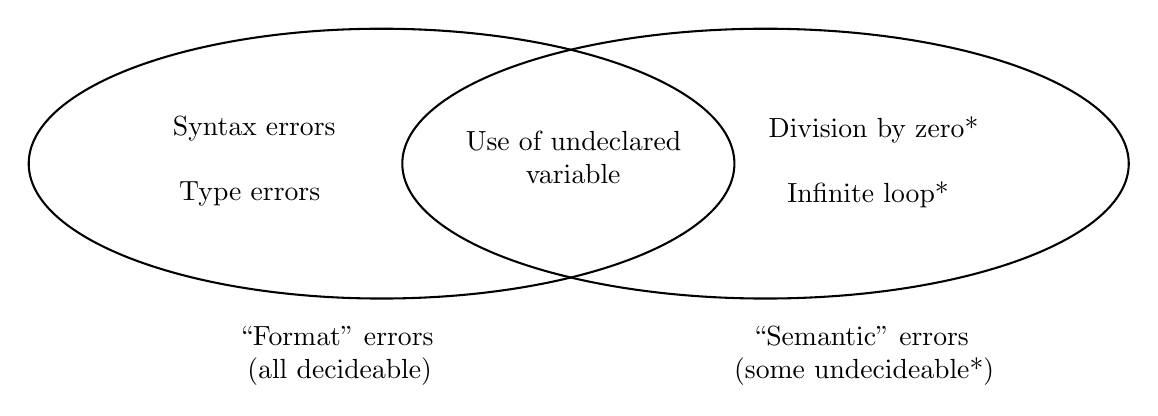
\begin{tikzpicture}[x=0.75pt,y=0.75pt,yscale=-1,xscale=1]
%uncomment if require: \path (0,300); %set diagram left start at 0, and has height of 300

%Shape: Ellipse [id:dp5326335354678456] 
\draw   (210,85) .. controls (210,49.1) and (288.35,20) .. (385,20) .. controls (481.65,20) and (560,49.1) .. (560,85) .. controls (560,120.9) and (481.65,150) .. (385,150) .. controls (288.35,150) and (210,120.9) .. (210,85) -- cycle ;
%Shape: Ellipse [id:dp904564307478004] 
\draw   (30,85) .. controls (30,49.1) and (106.11,20) .. (200,20) .. controls (293.89,20) and (370,49.1) .. (370,85) .. controls (370,120.9) and (293.89,150) .. (200,150) .. controls (106.11,150) and (30,120.9) .. (30,85) -- cycle ;

% Text Node
\draw (98,61) node [anchor=north west][inner sep=0.75pt]   [align=left] {Syntax errors};
% Text Node
\draw (351,162) node [anchor=north west][inner sep=0.75pt]   [align=left] {\begin{minipage}[lt]{120pt}\setlength\topsep{0pt}
\begin{center}
“Semantic" errors\\(some undecideable*)
\end{center}

\end{minipage}};
% Text Node
\draw (125,162) node [anchor=north west][inner sep=0.75pt]   [align=left] {\begin{minipage}[lt]{80pt}\setlength\topsep{0pt}
\begin{center}
“Format" errors\\(all decideable)
\end{center}

\end{minipage}};
% Text Node
\draw (101,92) node [anchor=north west][inner sep=0.75pt]   [align=left] {Type errors};
% Text Node
\draw (231,68) node [anchor=north west][inner sep=0.75pt]   [align=left] {\begin{minipage}[lt]{90pt}\setlength\topsep{0pt}
\begin{center}
Use of undeclared\\variable
\end{center}

\end{minipage}};
% Text Node
\draw (385,61) node [anchor=north west][inner sep=0.75pt]   [align=left] {Division by zero*};
% Text Node
\draw (394,92) node [anchor=north west][inner sep=0.75pt]   [align=left] {Infinite loop*};


\end{tikzpicture}

\caption{Format errors include syntax errors, type errors and some ``semantic'' errors as long as they are decideable.}
\label{fig:format-errors}
\end{figure}

\hypertarget{editors}{%
\subsubsection{Editors}\label{editors}}

\paragraph{Editors.}

These are programs for creating various data structures in the form of
files. Editors for 3D models, vector graphics, raster images, audio, and
video understand the file formats and strive to save only valid files.
It is usually not possible to even \emph{express} a structure in the
editor that contains a format error. Such cases are exceptional: for
example, a 3D scene might open without errors in another 3D editor, but
cause errors in a game engine according to the latter's additional
requirements---perhaps it expects specific objects in the scene named
\texttt{Player}, \texttt{Exit}, and so on. Nevertheless, for most
editors and most use cases, the consumer-side validity rules are in
harmony with the producer-side rules.

\paragraph{Text Editors.}

These are a type of editor for plain text files. However, they are
widely used to write code in programming languages, which have extra
syntax rules beyond the plain text format. Unlike most editors, text
editors \emph{can} save files that are invalid from the perspective of
their consumers under realistic use-cases. These syntax errors are then
discovered at the point of consumption.

\paragraph{Conclusion.}

The basic intuition behind Explicit Structure is the \emph{directness}
experienced in creation and programming. Almost every data structure in
computing has an editor with which one can manipulate the structure
directly, and when programming we can act as if data structures have
named parts that we can simply reference. This directness is interrupted
by the standalone exception of text editors (on the creation side) and
strings with machine-readable\footnote{We are unconcerned with strings
  that contain natural language simply to be echoed out to the user
  (e.g.~error messages). However, our ideas about Explicit Structure may
  be applicable to cases where software must parse and interpret natural
  language too.} implicit content (on the programming side).

\input{ch-analysis.tex}
\input{ch-tech-dims.tex}
\input{ch-state-first.tex}
\input{ch-bl.tex}
\joel{
\input{ch-related-work.tex}
\input{ch-future-work.tex}
\input{ch-conclusion.tex}
}

\chapter*{Appendices}
\todo{Structure this properly}
\appendix
%\input{appendix-misc.tex}
%\input{appendix-tech-dims.tex}
\input{appendix-all-dims.tex}
\input{appendix-bl.tex}

\printbibliography

\end{document}
